\KOMAoptions{paper=A3}
\recalctypearea
\subsection{Linear Feedback Shift Register}{\label{pp:linearfeedbackshiftregister}}
How does a computer generate truly random numbers? Computers are deterministic which means the actions it takes are predetermined. So it can't generate truly random numbers unless they observe some unpredictable data like noise. But we can still generate ``seemingly'' random numbers called \textbf{pseudorandom numbers}. One such approach is using Linear Feedback Shift Registers (LFSRs).

An LFSR is defined by
\begin{itemize}	
	\item $n$ state variables $x_1, x_2, x_3,\ldots, x_n$ (collectively called as the state of LFSR (``register'')) with their initial values (called taps) $t_1, t_2, t_3,\ldots, t_n$ ($t_i$ is 0 or 1).
	\item A feedback polynomial $c_1x^0 + c_2x^1 + c_3x^2 + \cdots +  c_nx^{n-1} + x^n$ ($c_i$ is 0 or 1) which updates the state of LFSR as follows
	\begin{itemize}
		\item $\op{next}(x_1, x_2, x_3,\ldots, x_{n-1}) = (x_2, x_3, x_4,\ldots, x_n)$ -- this is called ``shifting'' next value of $x_1$ becomes $x_2$, next value of $x_2$ becomes $x_3$, and so on.
		\item $\op{next}(x_n) =  c_1x_1 \oplus c_2x_2 \oplus \cdots \oplus c_{n-1}x_{n-1}\oplus c_nx_n$ where $\oplus$ is the binary \href{https://en.wikipedia.org/wiki/Exclusive_or}{xor} operator -- this is the ``linear feedback''.
	\end{itemize}
	\item The output bit is $x_1$
\end{itemize}
For example, consider a $3-$bit LFSR as shown in \ref{fig:lfsrintro}. Here, $(t_1,t_2,t_3)=(1,1,0)$ and $(c_1,c_2,c_3)=(1,0,1)$.\\
Next, the sequence generation is shown in \ref{fig:lfsrgeneration}. Here, the initial state $(1,1,0)$ becomes $(1,0,1\oplus0) = (1,0,0)$ and with similar updates, eventually the sequence repeats when the state becomes $(1,1,1)$ as next state will be $(1,1,1\oplus1) = (1,1,0)$.
\begin{figure}[H]
	\centering
	\begin{subfigure}[c]{0.4\linewidth}
		\centering
		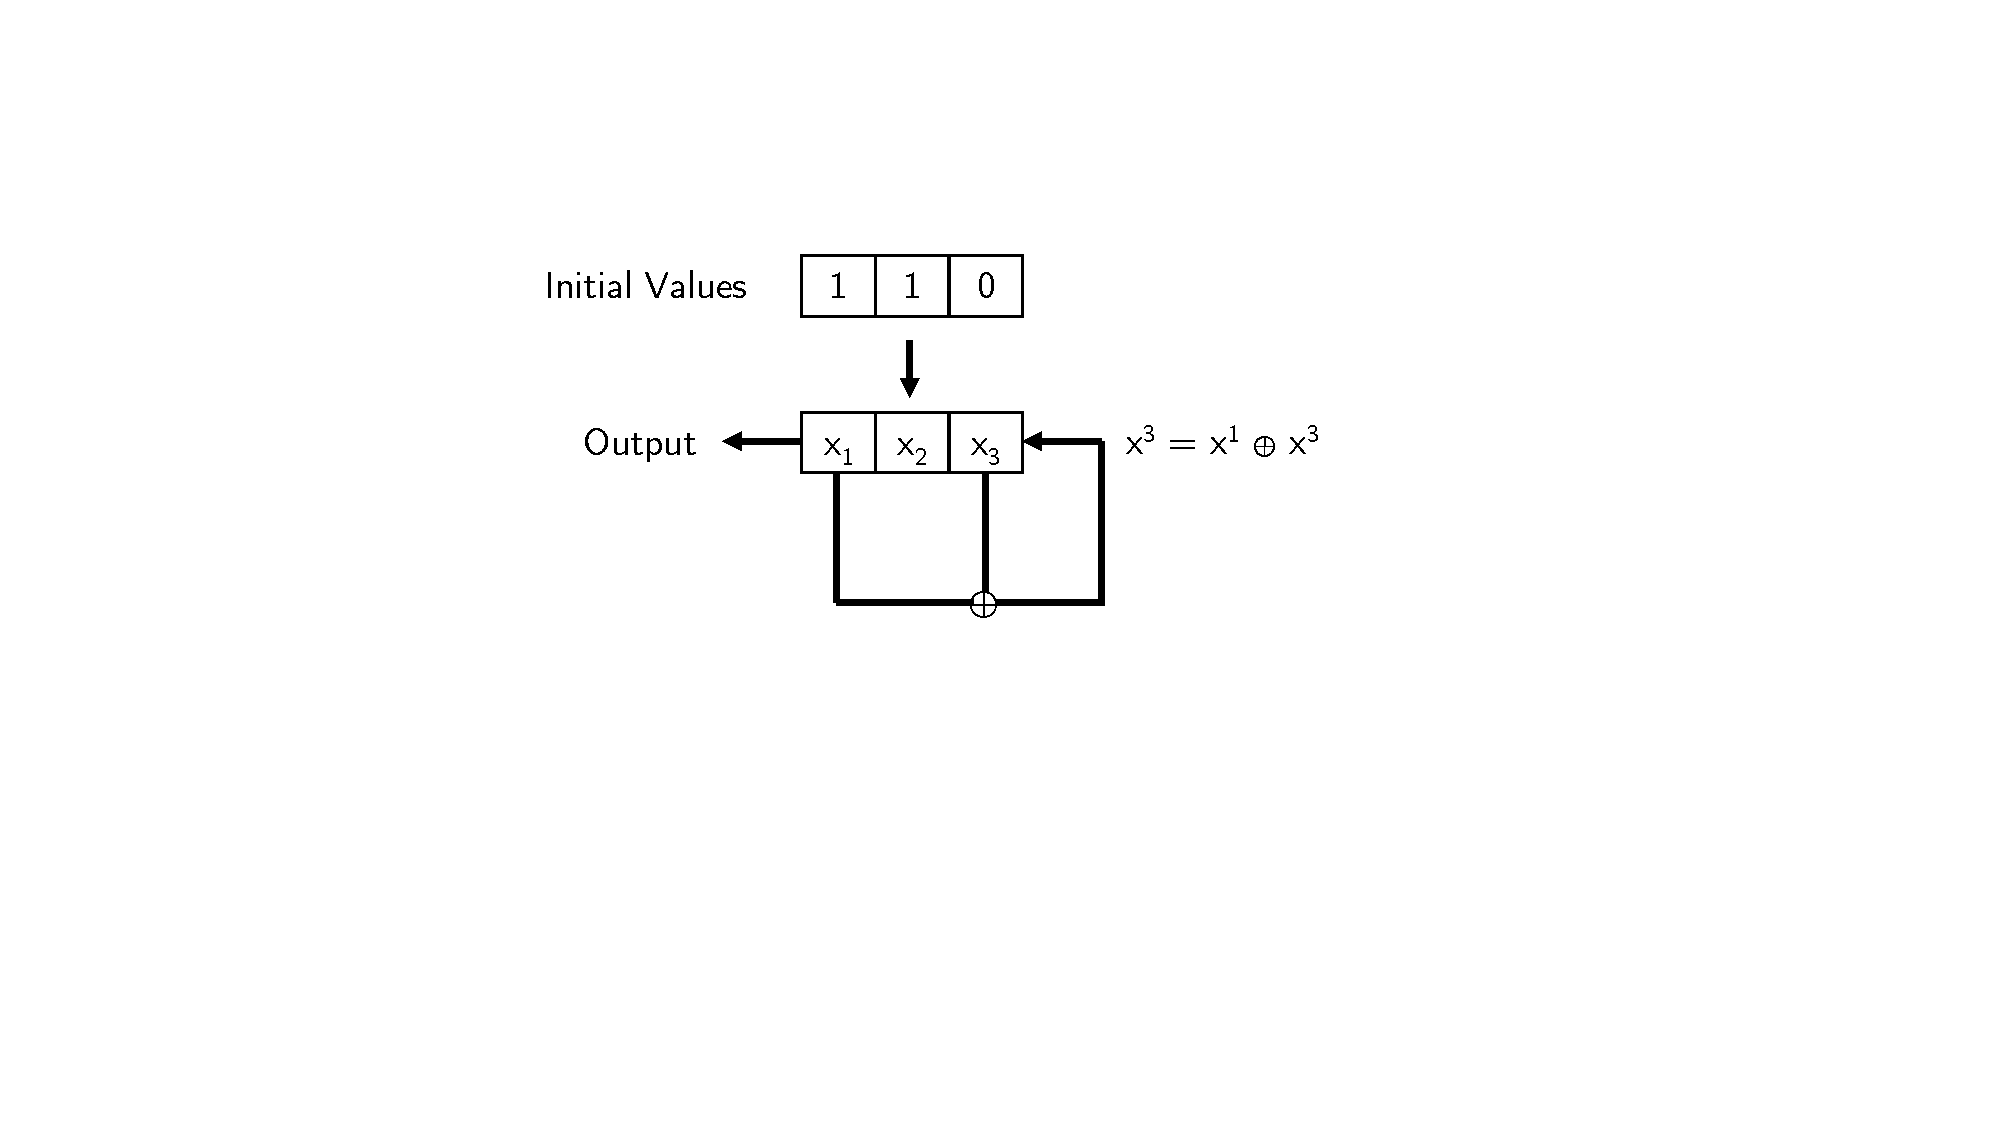
\includegraphics[width = \linewidth]{Linear Feedback Shift Register/Introduction.pdf}
		\caption{Given LFSR}
		\label{fig:lfsrintro}
	\end{subfigure}
	\begin{subfigure}[c]{0.45\linewidth}
		\centering
		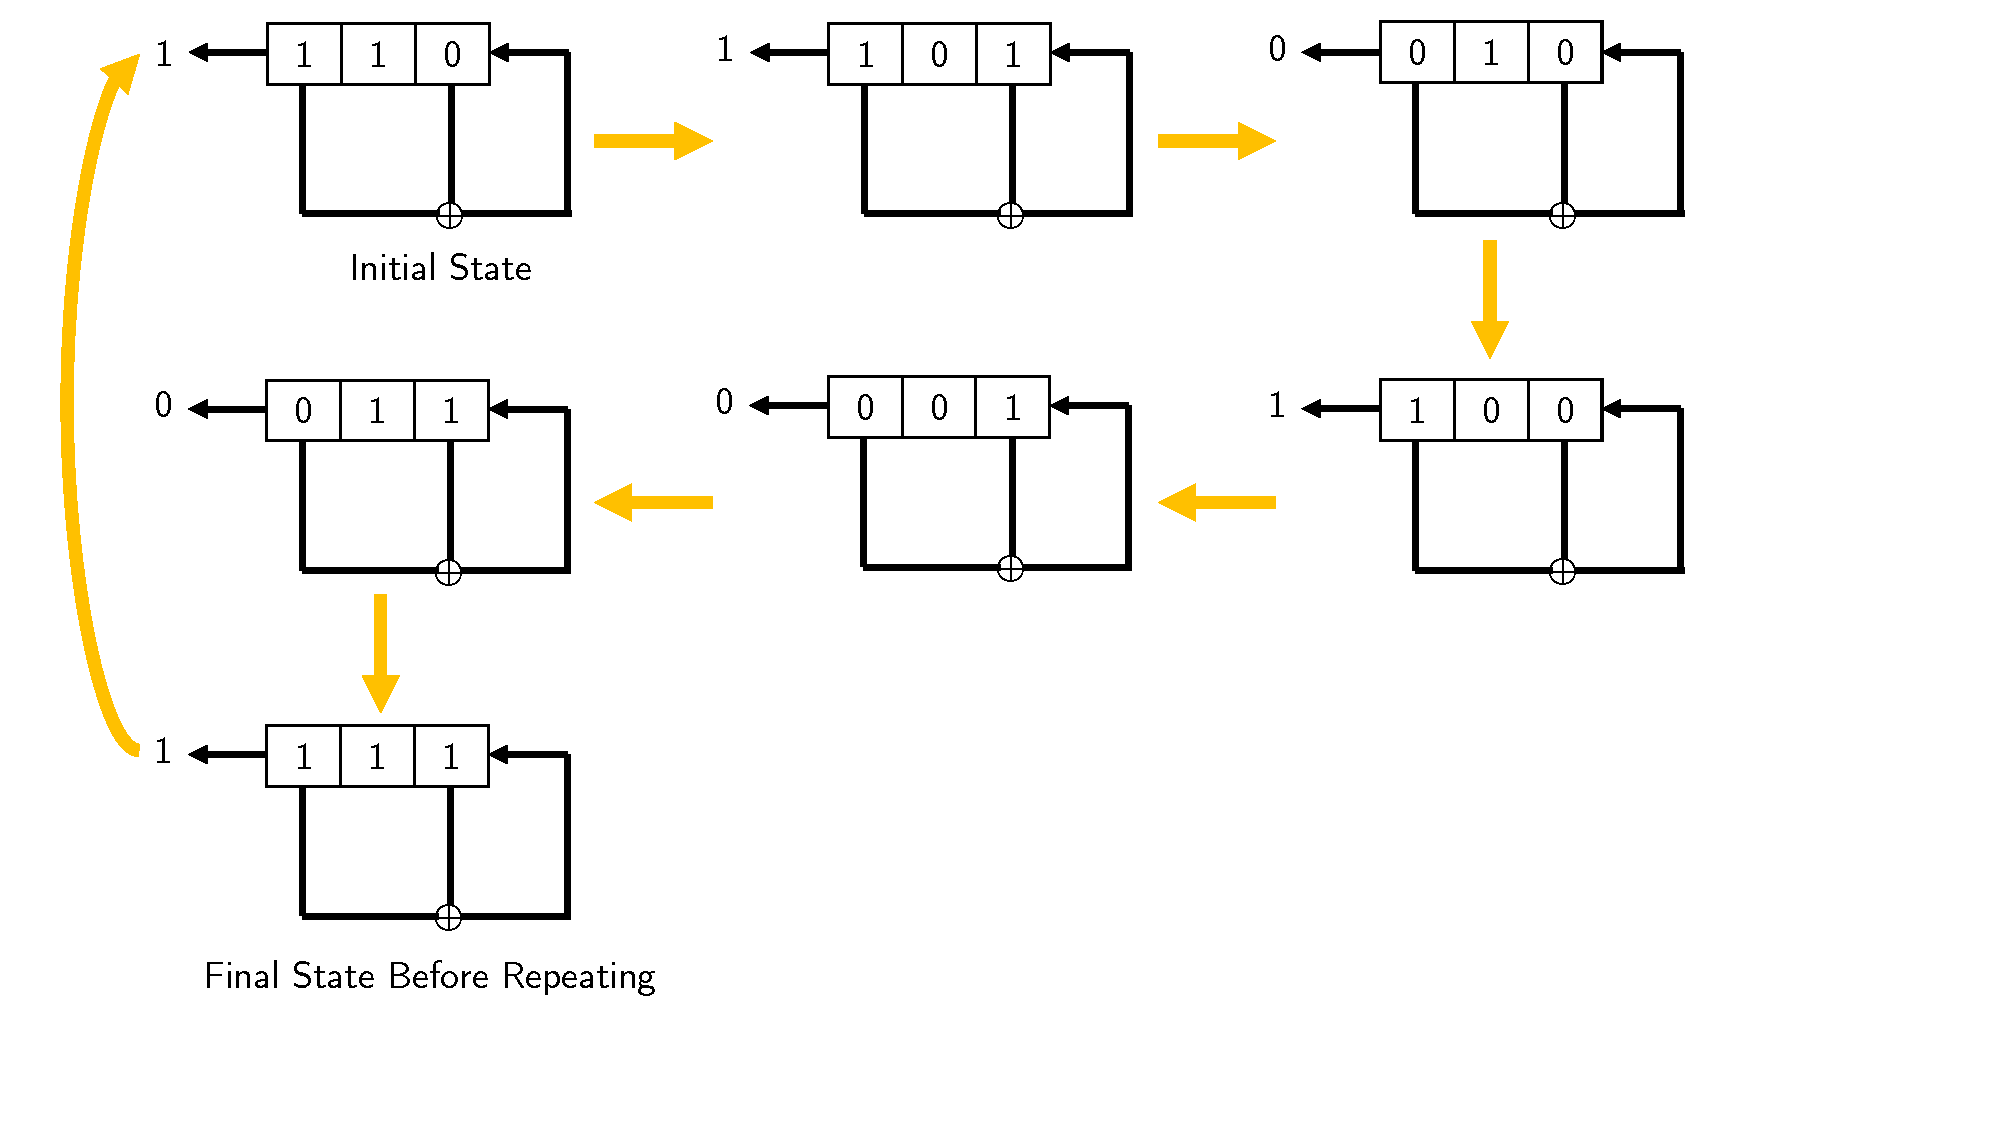
\includegraphics[width = \linewidth]{Linear Feedback Shift Register/Sequence Generation.pdf}
		\caption{The Generated Sequence is 11001001 repeating (follow the arrows)}
		\label{fig:lfsrgeneration}
	\end{subfigure}
	\caption{Linear Feedback Shift Register -- Working}
\end{figure}
\vspace{-2em}
\textbf{Problem Statement:}\\
A property of $n$ bit LFSR is that the output sequence it generates will start repeating in at most $2^{n-1}$ iterations called its period\footnote{Interestingly, there also exists a feedback polynomial which achieves this maximum period for every $n$.}.\\
Your task is to simulate an LFSR with a given initial state and feedback polynomial until it repeats and find its period\footnote{Is there a way to get the period of the sequence using just the feedback polynomial and without actually calculating sequence? The basis of this problem lie in the fascinating area of mathematics known as Abstract Algebra!
} in the process.
\begin{testcasesMore}
	{$t$ \hfill(number of test cases, an integer)\\
	$n_i\quad t_1\ t_2\ \cdots t_{n_i}\quad c_1\ c_2\ \cdots c_{n_i}$ \hfill($2n_i+1$ space seperated integers for each testcase)}
	{the output sequence generated by the given LFSR followed by the period of this output sequence\hfill(each iteration on a newline)}
	{$1 \leq n_i \leq 15$\\
	$t_i$ is either 0 or 1 and $c_1 = 1$\footnotemark,\ other $c_i$ are either 0 or 1\hfill(The LFSR will repeat from the beginning)}
	{1\quad 1 \quad 1\\2\quad1 0\quad1 0\\2 \quad 1 1 \quad 1 0\\2 \quad 1 1 \quad 1 1\\3 \quad 1 1 0 \quad 1 0 1\\5 \quad 1 0 1 0 0 \quad 1 0 0 1 0\\7 \quad 1 1 0 0 0 0 0 \quad 1 0 0 0 0 0 1}
	{1\quad1\\1 0\quad2\\1\quad1\\1 1 0\quad3\\1 1 0 1 0 0 1\quad7\\1 0 1 0 0 1 0 0 0 0 1 0 1 0 1 1 1 0 1 1 0 0 0 1 1 1 1 1 0 0 1\quad31\\1 1 0 0 0 0 0 1 0 0 0 0 0 0 1 1 1 1 1 1 1 0 1 0 1 0 1 0 0 1 1 0 0 1 1 1 0 1 1 1 0 1 0 0 1 0 1 1 0 0 0 1 1 0 1 1 1 1 0 1 1 0 1 0 1 1 0 1 1 0 0 1 0 0 1 0 0 0 1 1 1 0 0 0 0 1 0 1 1 1 1 1 0 0 1 0 1 0 1 1 1 0 0 1 1 0 1 0 0 0 1 0 0 1 1 1 1 0 0 0 1 0 1 0 0 0 0\quad127}
	{https://github.com/paramrathour/CS-101/tree/main/Test Cases/Linear Feedback Shift Register/Input.txt}
	{https://github.com/paramrathour/CS-101/tree/main/Test Cases/Linear Feedback Shift Register/Output.txt}
	{https://github.com/paramrathour/CS-101/tree/main/Starter Codes/Linear Feedback Shift Register.cpp}
\end{testcasesMore}
\footnotetext{This makes sure that the sequence will repeat from the beginning and will not have any non-periodic part. For example, $110101010\ldots$ (`10' repeating) is not possible if $c_1 = 1$.}
\begin{funvideo}
	\href{https://youtu.be/Ks1pw1X22y4}{Random Numbers with LFSR (Linear Feedback Shift Register) -- Computerphile}
\end{funvideo}
\KOMAoptions{paper=A4}
\recalctypearea